% Created 2023-11-24 Fri 23:24
% Intended LaTeX compiler: pdflatex
\documentclass[11pt]{article}
\usepackage[utf8]{inputenc}
\usepackage[T1]{fontenc}
\usepackage{graphicx}
\usepackage{longtable}
\usepackage{wrapfig}
\usepackage{rotating}
\usepackage[normalem]{ulem}
\usepackage{amsmath}
\usepackage{amssymb}
\usepackage{capt-of}
\usepackage{hyperref}
\usepackage{siunitx}
\author{Hankertrix}
\date{\today}
\title{Physics Magnetic Fields Cheat Sheet}
\hypersetup{
 pdfauthor={Hankertrix},
 pdftitle={Physics Magnetic Fields Cheat Sheet},
 pdfkeywords={},
 pdfsubject={},
 pdfcreator={Emacs 29.1 (Org mode 9.6.6)}, 
 pdflang={English}}
\begin{document}

\maketitle
\setcounter{tocdepth}{2}
\tableofcontents \clearpage
\section{Definitions}
\label{sec:org036dd9a}

\subsection{Right-hand grip rule}
\label{sec:orge9583e0}
The direction of the magnetic field generated by a current carrying conductor is given by the right-hand grip rule.

\begin{center}
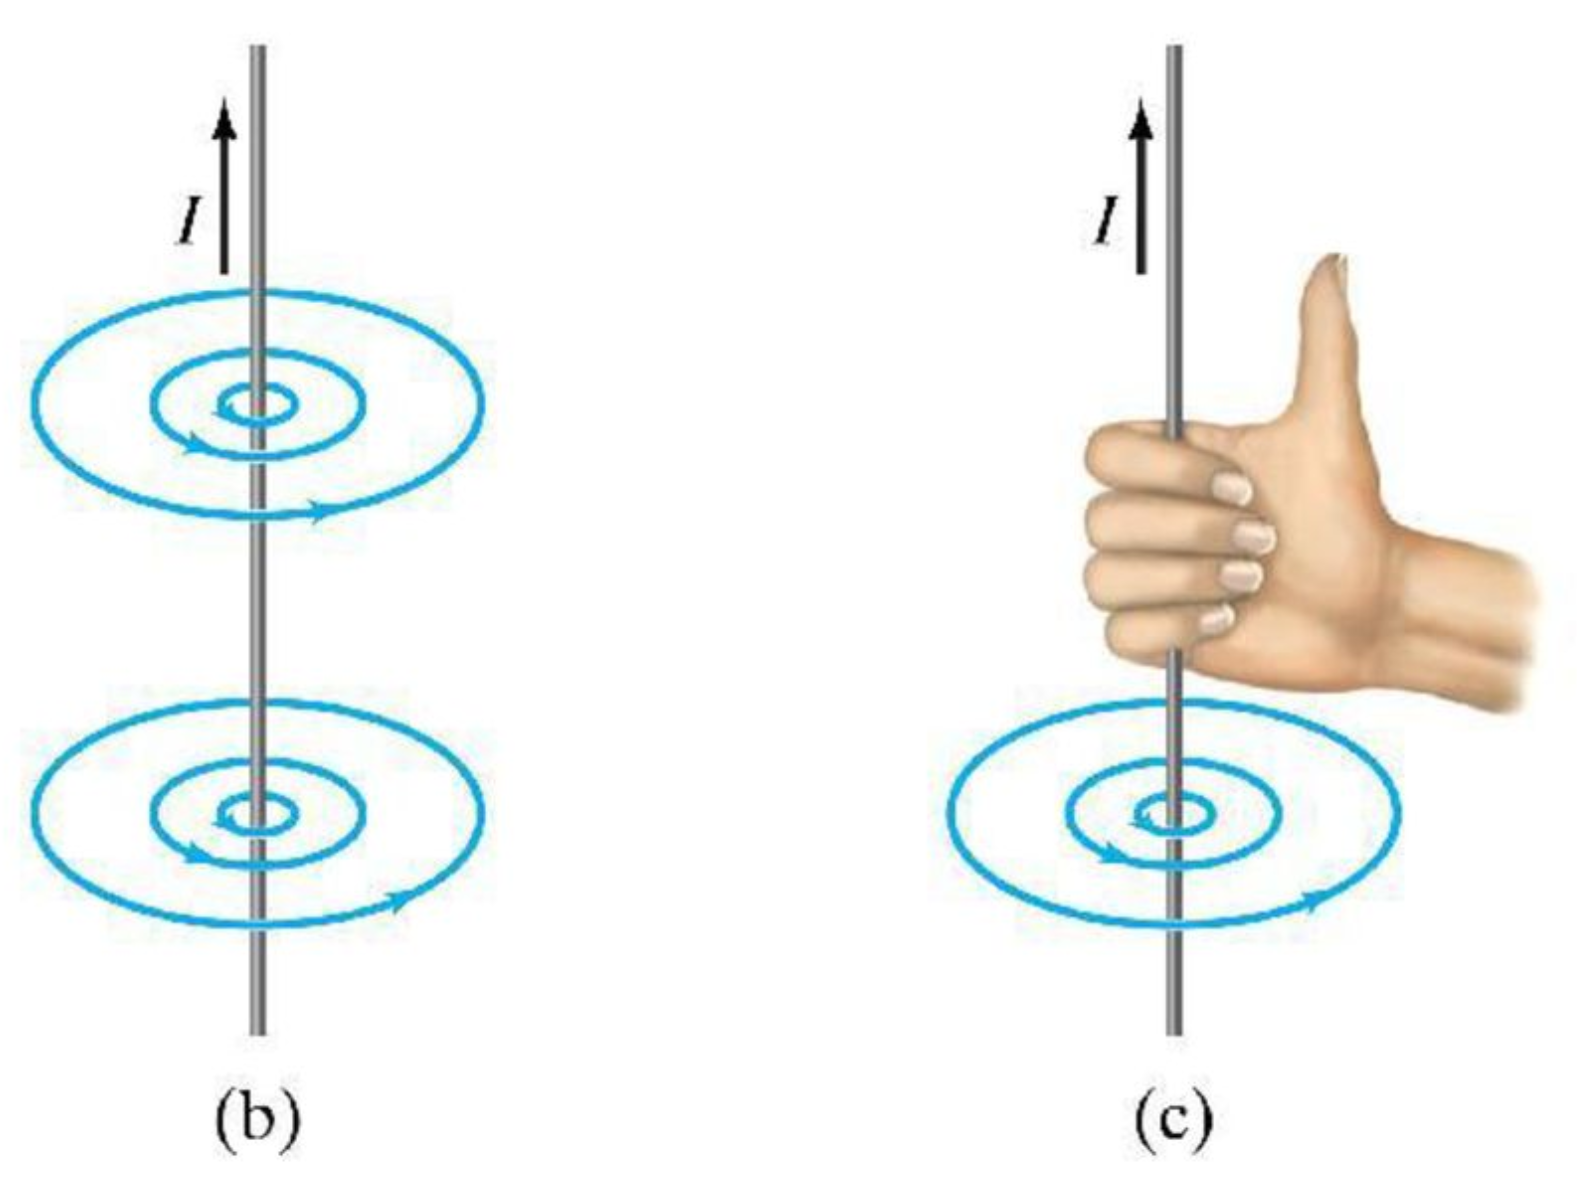
\includegraphics[scale=0.15]{./images/right-hand-grip-rule.png}
\end{center}

\subsection{Biot-Savart law}
\label{sec:org58793d4}

\subsubsection{Moving point charge}
\label{sec:org0758889}
The Biot-Savart law for point charges is:
\[\vec{\boldsymbol{B}} = \frac{\mu_0}{4 \pi} \frac{q \vec{\boldsymbol{v}} \times \hat{\boldsymbol{r}}}{r^2}\]

Where:
\begin{itemize}
\item \(\vec{\boldsymbol{B}}\) is the magnetic field due to a point charge with constant velocity.
\item \(\mu_0\) is the permeability of a vacuum, which is \(4 \pi \times 10^{-7} \ \unit{H.m^{-2}}\).
\end{itemize}

\begin{center}
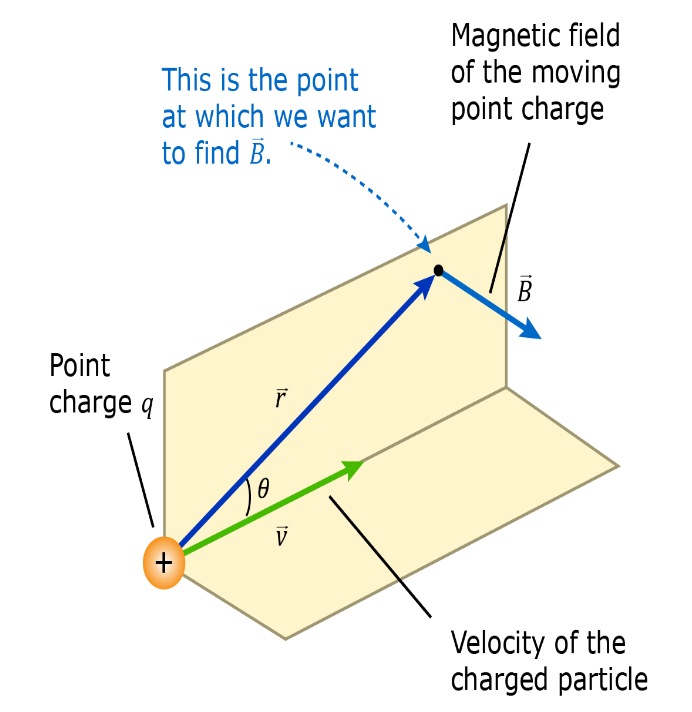
\includegraphics[scale=0.55]{./images/biot-savart-law-moving-charge.png}
\end{center}

\subsubsection{Current}
\label{sec:org82416c1}
For a current carrying wire, consider a small charge \(dq\) in a small length element of current carrying wire \(ds\) where the charge moves with velocity \(\vec{v}\). We can write:
\[dq \vec{v} = dq \frac{d \vec{s}}{dt} = I \, d \vec{s}\]

With the above equation, we have made the length element a vector, which has the direction as that of the current. Thus, each length element produces a magnetic field:
\[d \vec{\boldsymbol{B}} = \frac{\mu_0}{4\pi} \frac{I \, d \vec{s} \times \hat{\boldsymbol{r}}}{r^2}\]

Where:
\begin{itemize}
\item \(d \vec{\boldsymbol{B}}\) is the magnetic field due to an infinitesimal current element.
\item \(\mu_0\) is the permeability of a vacuum, which is \(4 \pi \times 10^{-7} \ \unit{H.m^{-2}}\).
\item \(I\) is the current.
\item \(d \vec{s}\) is the vector length of the current element. It points in the current direction.
\item \(\hat{\boldsymbol{r}}\) is the unit vector from the current element towards where the field is measured
\item \(r\) is the distance from the current element to where the field is measured.
\end{itemize}

\newpage

\subsection{Ampere's law}
\label{sec:org7dd2990}
Ampere's law states that the line integral of the total magnetic field is proportional to the algebraic sum of the currents.

\[\oint \vec{\boldsymbol{B}} \cdot d \vec{\boldsymbol{l}} = \mu_0 I_{encl}\]

Where:
\begin{itemize}
\item \(\oint \vec{\boldsymbol{B}} \cdot d \vec{\boldsymbol{l}}\) is the line integral around a closed path.
\item \(\vec{\boldsymbol{B}} \cdot d \vec{\boldsymbol{l}}\) is the scalar product of the magnetic field and the vector segment of the path.
\item \(\mu_0\) is the permeability of a vacuum, which is \(4 \pi \times 10^{-7} \ \unit{H.m^{-2}}\).
\item \(I_{encl}\) is the net current enclosed by the path.
\end{itemize}

Ampere's law is valid for conductors and paths of any shape. If the integral around the closed path is zero, it does not necessarily mean that the magnetic field is zero everywhere along the path, only that the total current through an area bounded by the path is zero.

\subsubsection{Convention}
\label{sec:orga145ecb}
Given a net enclosed current direction, we choose the direction of the path to be that path "curled around" by the fingers of the right hand when the thumb points in the direction of the net enclosed current.

\begin{center}
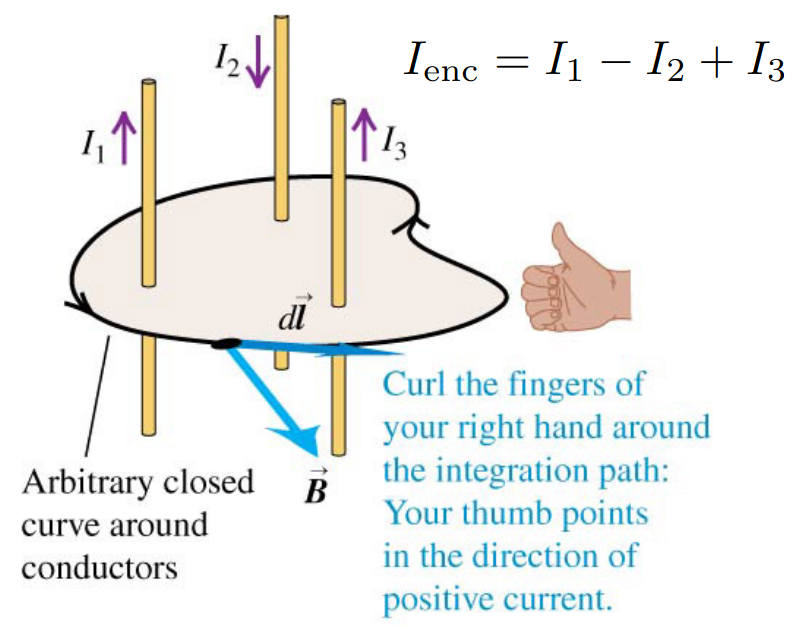
\includegraphics[scale=0.65]{./images/amperes-law.png}
\end{center}

\subsection{Magnetic flux}
\label{sec:org3e3af81}
\begin{align*}
\Phi_B &= \int B \cos \phi \, dA \\
&= \int B_{\perp} \, dA \\
&= \int \vec{\boldsymbol{B}} \cdot d \vec{\boldsymbol{A}}
\end{align*}

Where:
\begin{itemize}
\item \(\Phi_B\) is the magnetic flux through a surface.
\item \(B\) is the magnitude of the magnetic field \(\vec{\boldsymbol{B}}\).
\item \(\phi\) is the angle between \(\vec{\boldsymbol{B}}\) and the normal to the surface.
\item \(dA\) is the element of surface area.
\item \(B_{\perp}\) is the component of \(\vec{\boldsymbol{B}}\) perpendicular to the surface.
\item \(d \vec{\boldsymbol{A}}\) is the vector element of the surface area.
\end{itemize}

\subsection{Gauss' law}
\label{sec:org75d04a9}
As there is no magnetic monopoles to date, all magnetic field lines must form a closed loop. This means that the magnetic flux through any closed surface is zero, which is what Gauss' law states:
\[\oint \vec{\boldsymbol{B}} \cdot d \vec{\boldsymbol{A}} = 0\]

Where:
\begin{itemize}
\item \(\vec{\boldsymbol{B}}\) is the magnetic field.
\item \(d \vec{\boldsymbol{A}}\) is the vector element of the surface area.
\end{itemize}

\newpage

\subsection{Force on a moving charge in a magnetic field}
\label{sec:org7416b15}
\[\vec{\boldsymbol{F}} = q \vec{\boldsymbol{v}} \times \vec{\boldsymbol{B}}\]

Where:
\begin{itemize}
\item \(\vec{\boldsymbol{F}}\) is the magnetic force on a moving charged particle.
\item \(q\) is the particle's charge.
\item \(\vec{\boldsymbol{v}}\) is the particle's velocity.
\item \(\vec{\boldsymbol{B}}\) is the magnetic field.
\end{itemize}

The magnetic force on a charged particle is always perpendicular to its velocity and therefore its instantaneous displacement. Therefore, the magnetic force \textbf{does no work}.

\subsection{Lorentz force}
\label{sec:org823b419}
The combination of magnetic and electric forces is called the Lorentz force:
\[\vec{F} = q \vec{E} + q \vec{v} \times \vec{B}\]

\subsection{Force on a current in a magnetic field}
\label{sec:org2d7f624}
\[\vec{F} = I \vec{l} \times \vec{B}\]

Where:
\begin{itemize}
\item \(\vec{F}\) is the magnetic force on a current carrying wire.
\item \(I\) is the current.
\item \(\vec{l}\) is the length vector of the wire, which is in the direction of the current.
\item \(\vec{B}\) is the magnetic field.
\end{itemize}

\subsubsection{Fleming's left-hand rule}
\label{sec:org4b6e147}

\begin{center}
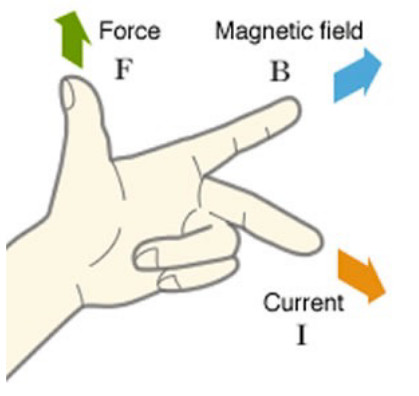
\includegraphics[scale=0.6]{./images/flemings-left-hand-rule.png}
\end{center}

\subsection{Magnetic field of a solenoid}
\label{sec:org594ef69}
\[B = \mu_0 n I\]

Where:
\begin{itemize}
\item \(B\) is the magnitude of the magnetic field.
\item \(\mu_0\) is the permeability of a vacuum, which is \(4 \pi \times 10^{-7} \ \unit{H.m^{-2}}\).
\item \(n\) is the number of coils of the wire around the solenoid.
\item \(I\) is the current.
\end{itemize}

\subsubsection{Increasing the magnetic field of a solenoid}
\label{sec:org00bb7f3}
The magnetic field of a solenoid can be increased by inserting a piece of soft iron:
\[B = \mu_0 n I \rightarrow B' = \mu nI\]

In this case, \(\mu \gg \mu_0\). When placed inside a magnetic field, the magnetic domains in the soft iron strengthen the already present magnetic field. Materials that increase the magnetic fields in this manner are described as ferromagnetic. Examples include soft iron, steel, cobalt and nickel.
\\[0pt]

There are also substances that contribute slightly to an external magnetic field (paramagnetic), \(\mu \gtrsim \mu_0\) and there are some which even expel external magnetic fields (diamagnetic), \(\mu < \mu_0\).

\subsection{Magnetic dipole moment}
\label{sec:orgd0b1727}
\[\vec{\mu} = NI \vec{A}\]

Where:
\begin{itemize}
\item \(\mu\) is the magnetic dipole moment.
\item \(N\) is the number of turns of the coil.
\item \(I\) is the current in each loop of the coil.
\item \(\vec{A}\) is the area vector.
\end{itemize}

\subsection{Torque experienced by a magnetic dipole}
\label{sec:org57301a3}
\begin{align*}
\vec{\tau} &= \vec{\mu} \times \vec{B} \\
&= NIA B \sin \theta
\end{align*}

Where:
\begin{itemize}
\item \(\vec{\tau}\) is the torque experienced by a magnetic dipole.
\item \(\vec{mu}\) is the magnetic dipole moment.
\item \(\vec{B}\) is the magnetic field vector.
\item \(N\) is the number of turns of the coil.
\item \(I\) is the current in each loop of the coil.
\item \(A\) is the surface area of the coil.
\item \(B\) is the magnitude of the magnetic field.
\item \(\theta\) is the angle between the magnetic field and the area vector.
\end{itemize}


\section{Magnetic field notation}
\label{sec:org4d0be23}
\begin{center}
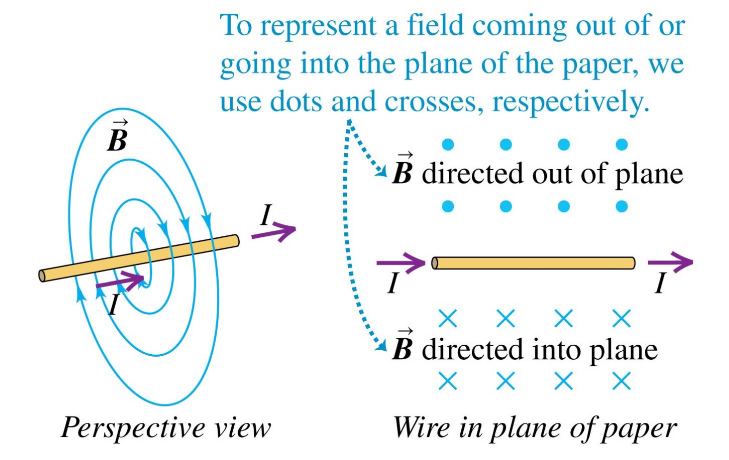
\includegraphics[width=.9\linewidth]{./images/magnetic-field-notation.png}
\end{center}


\section{Applications}
\label{sec:orga6a4cd1}

\subsection{Velocity selector}
\label{sec:orgd7bef26}

\begin{center}
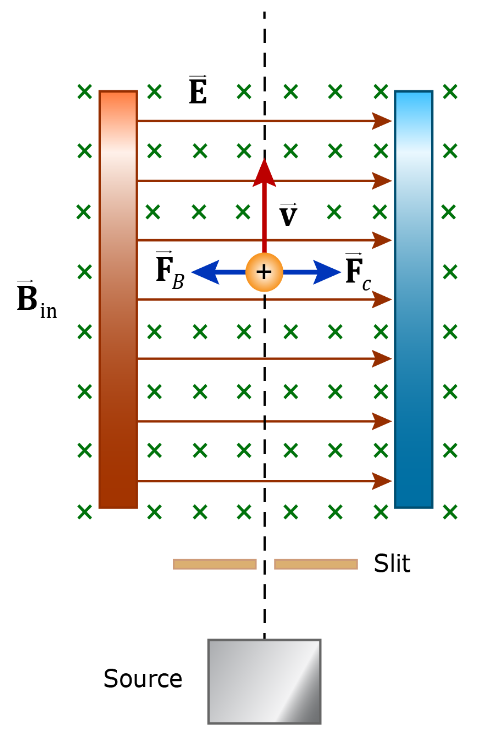
\includegraphics[scale=0.7]{./images/velocity-selector.png}
\end{center}

When a charged particle is injected into a region with perpendicular \(\boldsymbol{E}\) and \(\boldsymbol{B}\) fields, it feels the electric and magnetic forces.
\\[0pt]

In this set up, when no deflection is produced, it means that the electric and magnetic forces balance:
\[F_E = F_B\]
\[qE = qv B_{in}\]
\[\therefore v = \frac{E}{B_{in}}\]

Since \(E\) and \(B\) are controllable, this device can be used to select for desired velocities.

\subsection{Mass spectrometer}
\label{sec:orgc89838a}

\begin{center}
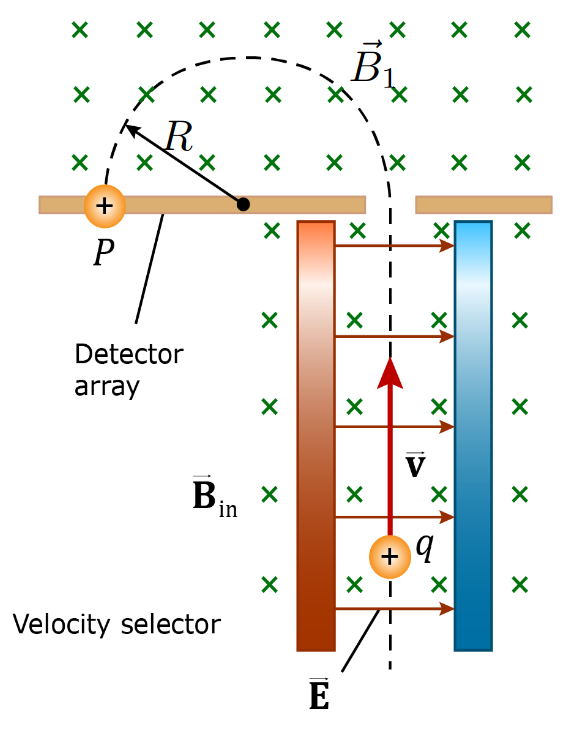
\includegraphics[scale=0.9]{./images/mass-spectrometer.png}
\end{center}

When charged particles have been passed through a velocity selector (bottom), and then injected into a region with a magnetic field (top), it moves in a circle and the radius of curvature can be measured. It is given by:
\begin{align*}
\frac{q}{m} &= \frac{v}{RB_1} \\
\frac{q}{m} &= \frac{E}{B_{in}} \frac{1}{RB_1} \\
m &= \frac{B_{in} B_1 Rq}{E}
\end{align*}

If the charge is known, then the mass can be determined.

\subsection{Hall effect}
\label{sec:org2ef3700}
\begin{center}
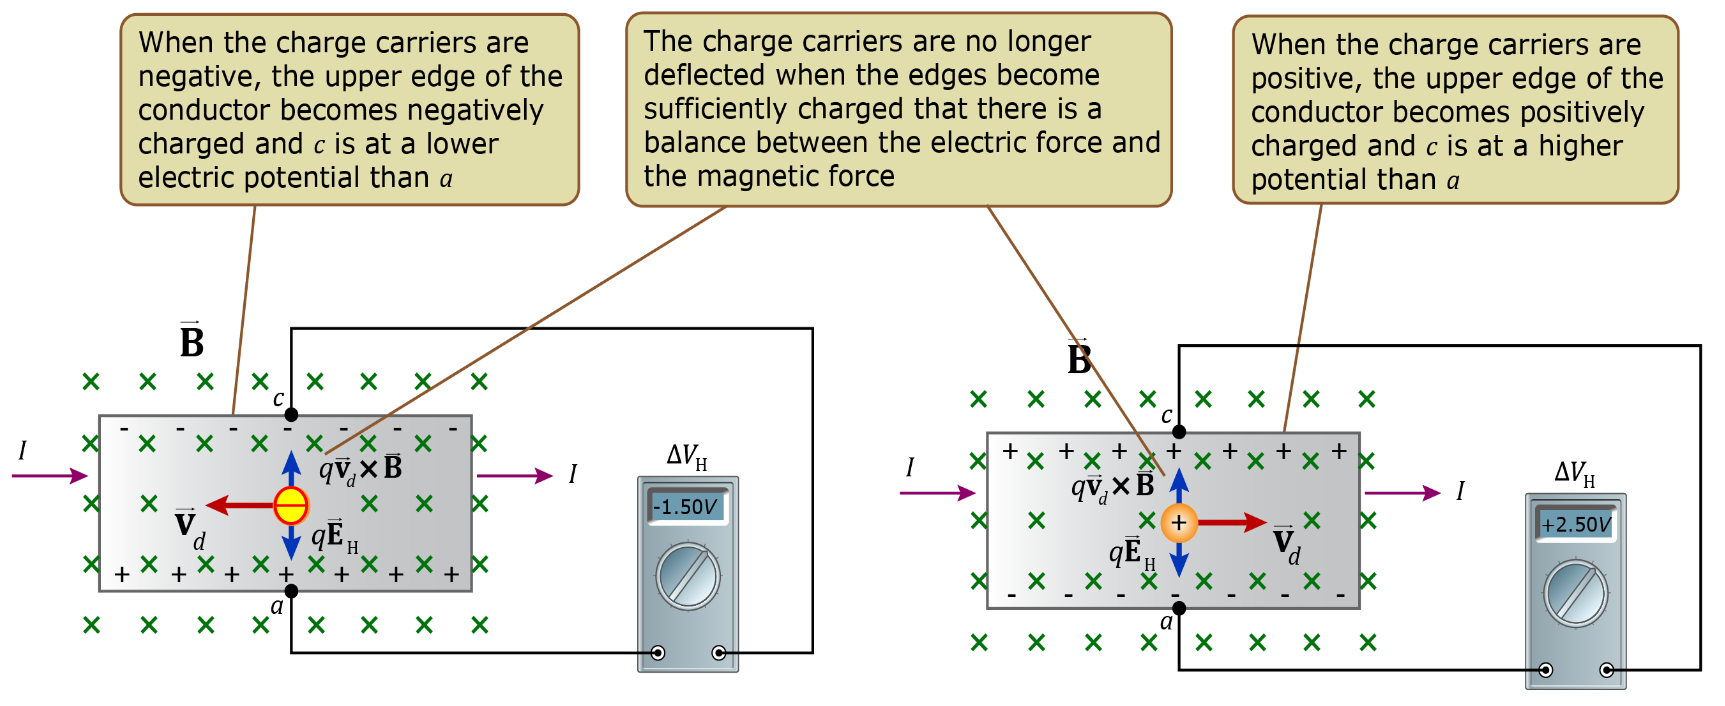
\includegraphics[width=.9\linewidth]{./images/hall-effect.png}
\end{center}

At steady state, magnetic force balances electric force, so the charge carriers move straight and are no longer deflected:
\[qE_H = qv_d B\]

If \(d\) is the width of the conductor, the Hall voltage is:
\[\Delta V_H = E_H d = v_d Bd\]

Where:
\begin{itemize}
\item \(d\) is the length \(ac\) in the diagram.
\item \(\Delta V_H\) is the Hall voltage.
\item \(B\) is the magnetic field.
\item \(v_d\) is the drift velocity.
\end{itemize}

\textbf{The sign of Hall voltage \(\boldsymbol{\Delta V_H}\) gives us the sign of the charge carriers.}
\end{document}